\documentclass[12pt,a4paper]{article}
\usepackage[utf8]{inputenc}
\usepackage[portuguese]{babel}
\usepackage{graphicx, hyperref, multicol, caption, verbatim}

\addtolength{\oddsidemargin}{-0.5in}
\addtolength{\evensidemargin}{-0.5in}
\addtolength{\textwidth}{1in}

\newenvironment{Figure}
  {\par\medskip\noindent\minipage{\linewidth}}
  {\endminipage\par\medskip}

\title{Relatório 2º Projeto de IA}
\author{Grupo 74 \\\\ Daniel Fernandes 86400 \& Francisco Sousa 86416}
\begin{document}
\maketitle
\begin{multicols}{2}
	\section{Introdução}
	Neste projecto vamos testar alguns algoritmos que lidam com a incerteza no
	mundo. Iremos testar métodos de modelação e inferência com redes Bayesiana,
	bem como métodos de aprendizagem por interação com o mundo.

	\section{Redes Bayesianas}
	%Para efeitos deste projeto as redes serão acíclicas.
	%Para o processo de inferência o algoritmo de eliminação não é necessário
	%mas discussão da diferença entre eles

	Foi implementada uma rede Bayesiana acíclica representada pela classe BN e os seus nodes pela classe Node.

	%No relatório deve incluir-se:
	%• descrição crítica dos resultados pedidos
	%• descrição dos métodos implementados incluindo vantagens/desvantagens e limitações
	%• discussão da complexidade computacional e possíveis métodos alternativos
	\subsection{Resultados}
	Os resultados pedidos estão de acordo com os resultados obtidos. Estes parecem, portanto, corretos. 

	\subsection{Métodos Implementados}
	\subsubsection{classe Node}
	A classe representa um Node da rede Bayesiana e contêm a tabela de probabilidades de acordo com a vericidade dos pais e uma lista destes.
	\paragraph{computeProb}
	Na classe Node apenas foi implementado o método computeProb que retorna a probabilidade do acontecimento do Node ser \textit{false} e de ser \textit{true} de acordo com a evidência dada.
	A complexidade deste método é O(\textit{no. parents}), sendo \textit{no. parents} o número de pais do Node.

	\subsubsection{classe BN}
	A classe BN representa uma rede Bayesiana e é composta por uma lista de Nodes e o grafo da rede, contendo os pais de cada Node.
	\paragraph{computeJointProb}
	Calcula a probabilidade conjunta da rede tendo em conta a evidência dada. É usada o método computeProb da classe Node
	A evidência não pode ter elementos desconhecidos.
	A complexidade deste método é O($n^2$), sendo $n$ o número de nodes da rede Bayesiana.
	\paragraph{substituteUnknowns}
	Método auxiliar a \textit{computeUnknownJointProb} que, dado uma evidência com $x$ acontecimentos desconhecidos e um conjunto de $x$ de valores (0 ou 1), retorna a evidência com os valores desconhecidos substituídos pelos novos valores dados.
	A complexidade deste método é O(\textit{no. desc}), sendo \textit{no. desc} o número de valores desconhecidos na evidência.
	\paragraph{computeUnknownJointProb}
	Método auxiliar a \textit{computePostProb} que, dada uma evidência com valores desconhecidos, gera todas as possibilidades dessa evidência sem valores desconhecidos e calcula a probabilidade conjunta, usando \textit{computeJointProb}.
	A complexidade deste método é O($2^m * n^2$), sendo $m$ o número de elementos desconhecidos e $n$ o número de nodes da rede Bayesiana. 
	\paragraph{computePostProb}
	Calcula a probabilidade a-posteriori da variável $x$ indicada na evidência (por -1). Usa \textit{computeUnknownJointProb} para calcular as probabilidades conjuntas para o caso de $x$ ser \textit{true} e para o caso de ser \textit{false}.
	De seguida usa a fórmula da probabilidade a-posteriori para a calcular e esta é retornada.
	A complexidade deste método é a mesma de \textit{computeUnknownJointProb}, ou seja, O($2^m * n^2$), sendo $m$ o número de elementos desconhecidos e $n$ o número de nodes da rede Bayesiana.
	\section{Aprendizagem por Reforço}
	
	\subsection{Representação gráfica}
	\paragraph{Ambiente 1}
	%Para cada um dos ambientes, e por inspecção das trajectórias, fazer uma representação
	%gráfica do ambiente no qual o agente se move (1val).
	%Descrição do forma como o agente se move ( Qual é o impacto de cada acção em cada estado )? (1val)
	
	A representação gráfica do primeiro ambiente está na figura \ref{amb1},
	sendo os estados representados e numerados pelos quadrados amarelos, e
	as ações possíveis em cada estado representadas e numeradas pelas setas.
	
	\begin{Figure}
		\centering
		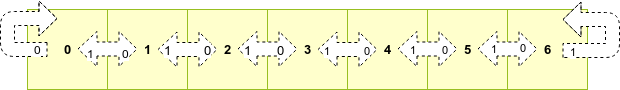
\includegraphics[width=1\textwidth]{ambiente1}
		\captionof{figure}{Rep. gráfica do ambiente 1}
		\label{amb1}
	\end{Figure}

	\paragraph{Ambiente 2}

	A representação gráfica do segundo ambiente está na figura \ref{amb2},
	com a mesma representação que a figura anterior.
	
	\begin{Figure}
		\centering
		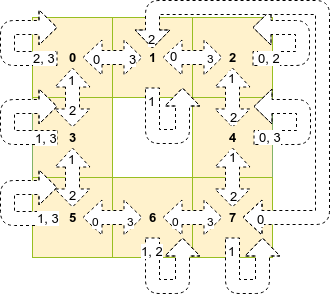
\includegraphics[width=1\textwidth]{ambiente2}
		\captionof{figure}{Rep. gráfica do ambiente 2}
		\label{amb2}
	\end{Figure}
	
	%Descrever qual a função de recompensa? (1val)
	\subsection{Função de recompensa}
	\paragraph{Ambiente 1}
	Para este ambiente, a função de recompensa, dado um estado inicial \textit{s}, é
	\begin{verbatim}
			def R(s):
			  if s == 0 or s == 6:
			    return 1
			  else:
			    return 0
	\end{verbatim}

	\paragraph{Ambiente 2}
	Para este ambiente, a função de recompensa, dado o mesmo estado inicial
	\textit{s}, é
	\begin{verbatim}
			def R(s):
			  if s == 7:
			    return 0
			  else:
			    return -1
	\end{verbatim}

	
	%Qual é a politica óptima? (1val)
	\subsection{Política Ótima}
	A política de \textit{exploration} é usada para descobrir o mundo e as várias
	trajetórias possíveis. A política de \textit{exploitation} toma vantagem
	dos dados já adquiridos para cada ação em cada estado, e faz as trajetórias
	que resultam em maior benefício, sendo a política ótima.

	\subsection{Resultados}
	Os resultados pedidos são uma boa aproximação da realidade e das
	soluções ótimas, variando sempre de iteração em iteração devido à
	utilização de valores aleatórios.
	
	\subsection{Métodos Implementados}
	\paragraph{traces2Q}
	Esta função calcula a máxima recompensa esperada para cada ação, em
	cada estado, usando o algoritmo de \textit{QLearning}.
	A complexidade desta é de O(${S * A}$), para \textit{S} estados e
	\textit{A} ações.

	\paragraph{policy}
	Esta função returna uma ação possível a fazer, dado um estado atual
	e uma política (\textit{exploration} ou \textit{exploitation}).

	%No relatório deve incluir-se também:
	%• descrição crítica dos resultados pedidos
	%• descrição dos métodos implementados incluindo vantagens/desvantagens e limitações
	%• discussão da complexidade computacional e possíveis métodos alternativos

	\section{Conclusão}
	Isto são resultados interessantes.

\end{multicols}
\end{document}